\section{Yksikkötestityökalujen vertailua}

Androidin yksikkötestaustapa on tehdä JUnit-testejä Androidin oman AndroidUnitTestCase-luokan aliluokkana. Nämä testit ajetaan emulaattorissa Dalvik-ympäristössä. Tässä tavassa on kaksi heikkoutta, joiden takia on kehitetty myös kolmansien osapuolien yksikkötestityökaluja Android-ympäristöön. Ensinnäkin testien ajaminen emulaattorissa on hitaampaa, kuin jos niitä voisi ajaa suoraan tavallisessa Javan virtuaalikoneessa JUnit-testeinä. Toiseksi muutkaan testauksen apuna käytettävät työkalut, kuten jäljittelijä-työkalut, eivät välttämättä toimi ongelmitta Dalvik-ympäristössä. Tässä luvussa vertailen Android-sovelluksen yksikkötestausta AndroidUnitTestCasella ja suosituimmalla Javan virtuaalikoneessa pyörivällä vaihtoehdolla: Robolectricillä. Tavoitteena on selvittää, voiko Robolectricillä helposti korvata Androidin oman yksikkötestikehyksen ja pitääkö Robolectricin lupaus nopeammasta testien suoritusajasta paikkansa.

Android-sovellusten yksikkötestauksessa kiinnostavaa on nimenomaan Androidin kirjastoluokista perivien keskeisten komponenttien testaus. Sovelluksessa mahdollisesti olevat muut kuin Androidin kirjastoluokista perivät luokat on helppo testata tavanomaisilla Javan yksikkötestityökaluilla ilman erityisesti Androidille tarkoitettuja työkaluja samaan tapaan kuin muutkin Java-sovellukset.

Yksikkötestityökalujen testaukseen sovellan luvussa \ref{test_criteria} esiteltyjä kriteerejä. Tärkein kriteeri on työkalujen toiminnallisuus: mitä niillä pystyy testaamaan, ja miten ne kommunikoivat testattavan sovelluksen kanssa. Yksikkötestityökaluissa toisena tärkänä kriteerinä pidän testien ajonopeutta, koska testivetoisessa kehityksessä yksikkötestejä ajetaan jatkuvasti ja jos testien ajoa joutuu odottamaan pitkään, koko kehityssykli hidastuu. Koska molemmat testattavat työkalut ovat JUnit-pohjaisia, niiden työkalutuki on käytännössä identtinen. Androidin yksikkötestityökalut tulevat luonnollisesti Android-kehyksen mukana, mutta Robolectric pitää erikseen asentaa, joten tämä vaikeuttaa Robolectricin käyttöönottoa. Molemmat työkalut ovat minulle uusia, joten arvioin subjektiivisesti työkalujen oppimisen helppoutta sekä testien kirjoitusnopeutta.

Ensimmäisessä aliluvussa esitellään lyhyesti Robolectric. Toisessa aliluvussa tutustutaan aiempaan tutkimukseen Androidin yksikkötestityökaluista. Seuraavassa aliluvussa esittelen testiprojektin, jota käytän testityökalujen testaamiseen. Neljännessä aliluvussa käsitellään Robolectricin asentamista. Viidennessä aliluvussa vertailen Robolectriciä ja AndroidUnitTestCasea testiprojektin elinkaarimetodien testauksessa. Kuudennessa aliluvussa vertaillaan työkalujen toimintaa jäljittelijäkehyksen kanssa. Seuraavassa aliluvussa vertaillaan työkalujen ajonopeuksia. Kahdeksannessa aliluvussa pohditaan Android-sovelluksen yksikkötestauksen haasteita ja viimeisessä aliluvussa analysoin testien tuloksia.

\subsection{Robolectric}

Robolectric on yksikkötestaustyökalu, jonka tarkoitus on mahdollistaa Android-koodin yksikkötestaus suoraan ohjelmointiympäristössä Javan virtuaalikoneessa ilman emulaattoria. Tarkoitus on mahdollistaa nopea tdd-sykli ja helpompi integrointi jatkuvan integroinnin palveluihin. Normaalisti Android-kirjaston luokat palauttavat kutsuttaessa ohjelmointiympäristöstä ajoaikaisen poikkeuksen, mutta Robolectric korvaa nämä luokat varjototeutuksilla, jotka palauttavat poikkeuksen sijaan tyhjän oletusvastauksen, kuten null, 0 tai false, tai jos Robolectricissa on kyseistä metodia varten olemassa varjototeutus, se palauttaa toteutuksen määrittelemän paluuarvon.

Robolectricin varjoluokkien käytön vaihtoehtona on jonkin jäljittelijäkehyksen käyttäminen Androidin kirjaston korvaamiseen, mutta tämä tapa kirjoittaa testejä on hyvin työläs, koska koodirivejä kertyy väistämättä paljon. Lisäksi tällöin testejä kirjoitettaessa täytyy tuntea testattavan metodin toiminta hyvin tarkasti, jotta jäljittelijätoteutukset saadaan kirjoitettua. Robolectricin varjoluokat mahdollistavat enemmän musta laatikko -tyyppisen testauksen \cite{robolectric}.

\subsection{Aiempaa tutkimusta}

Sadeh et al. vertasivat Androidin aktiviteettien yksikkötestausta JUnitilla, Androidin omilla yksikkötestityökaluilla sekä Robolectricilla \cite{sadehetal11}. JUnitilla testattaessa ongelmaksi muodostui, että ohjelmakoodia jouduttiin melko rajusti muokkaamaan, jotta luokkien yksikkötestaus onnistui. Tämä tekee ohjelman ylläpidon vaikeaksi. JUnitin hyvä puoli oli erittäin nopea testien ajonopeus. Robolectricillä testien tekeminen taas oli lähes yhtä helppoa kuin Androidin omilla työkaluilla. Androidin työkaluihin verrattuna Robolectricin vahvuudet olivat virhepaikkojen paikantamisen helppous ja testien suoritusnopeus. Robolectric-testit ajautuivat viisi kertaa nopeammin kuin Androidin työkaluilla ajetut testit, koska Androidin työkaluilla kirjoitetut testit ajetaan Dalvik-emulaattorilla, Robolectric taas suoraan Javalla. Androidin omien työkalujen suurin vahvuus oli testien kirjoittamisen helppous.

Sadeh et al. eivät käyttäneet JUnit-testeissään mitään jäljittelijätyökalua, joten testeissä testiluokan riippuvuudet jäljiteltiin tekemällä niistä staattisia sisäluokkia testiluokan sisään. Tämä vaatii paljon koodia ja vaikutti osaltaan siihen, miksi puhdas JUnit-testi näytti niin hankalalta. Androidin kirjastoluokat on pakko eristää testattavasta luokasta Javan virtuaalikoneella testattaessa, koska Androidin kehitysympäristössä käytettävä paketti ei sisällä varsinaisesti luokkien sisältöä, vaan vain niiden luokkien julkiset rajapinnat, jolloin kehitystyökalut osaavat auttaa niiden käytössä, mutta varsinaista toteutusta ei ole.

Jeon \& Foster \cite{troyd} mainitsevat Robolectricin vahvuudeksi sen, että se pyörii Javan virtuaalikoneessa ja näin ohittaa testeistä hitaan vaiheen, jossa sovellus pitää kääntää emulaattorille tai laitteelle testattavaksi. Robolectric ei heidän mielestään kuitenkaan sovellu kokonaisten sovellusten testaamiseen, koska sen varjoluokat eivät toteuta Androidin komponenteista kuin osan.

Allevato \& Edwards \cite{robolift} käyttivät Robolectriciä opetuskäyttöön tarkoitetun RoboLIFT-työkalun kehitykseen. Robolectric auttoi heitä ohittamaan emulaattorin käytön ja nopeuttamaan opiskelijoiden testisykliä ja automaattista arviointialgoritmia. Tässä käytössä Robolectricin ongelma oli, että se ohittaa käyttöliittymän piirtämisen kokonaan ja muunmuassa näkymien onDraw()-metodia ei kutsuta ollenkaan. Tämän seurauksena esimerksi näkymän leveys on aina 0 pikseliä, jolloin sellaiset testit, joilla haluttiin klikata näytöllä johonkin suhteelliseen kohtaan (vaikkapa keskelle) eivät toimineet oikein.

\subsection{Testiprojekti}

\begin{figure}[h]
\centering
\fbox{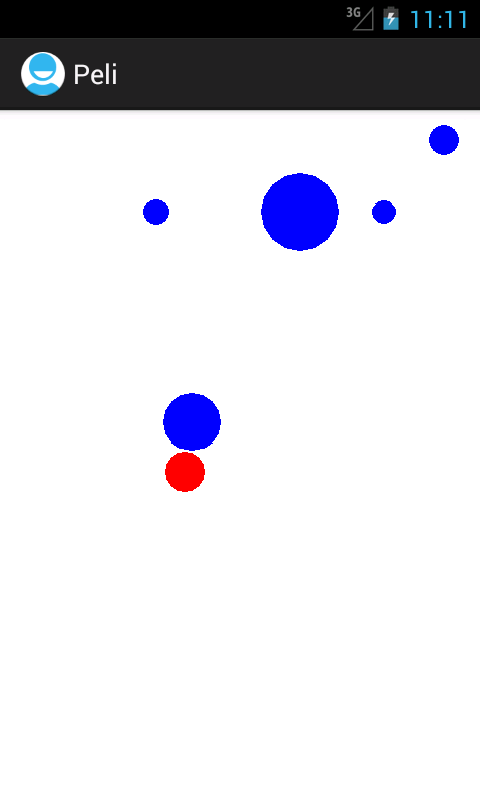
\includegraphics[width=60mm]{peli_screenshot.png}}
\caption{Ruutukaappaus testiohjelman pelinäkymästä} \label{peli_screenshot}
\end{figure}

Yksikkötestaustyökaluja testasin itse tehdyllä demoprojektilla. Kyseessä on yksinkertainen peli, jonka pelinäkymästä on ruutukaappaus kuvassa \ref{peli_screenshot}. Pelissä ohjataan kosketusnäytöllä painamalla punaista palloa ja pyritään väistämään ympäriinsä pomppivia sinisiä palloja. Kun peli päättyy, palataan takaisin päänäkymään, josta on ruutukaappaus kuvassa \ref{mainactivity}. Tästä näkymästä voi aloittaa uuden pelin ja lisäksi näkee, montako sekuntia edellinen peli kesti.

\begin{figure}[h]
\centering
\fbox{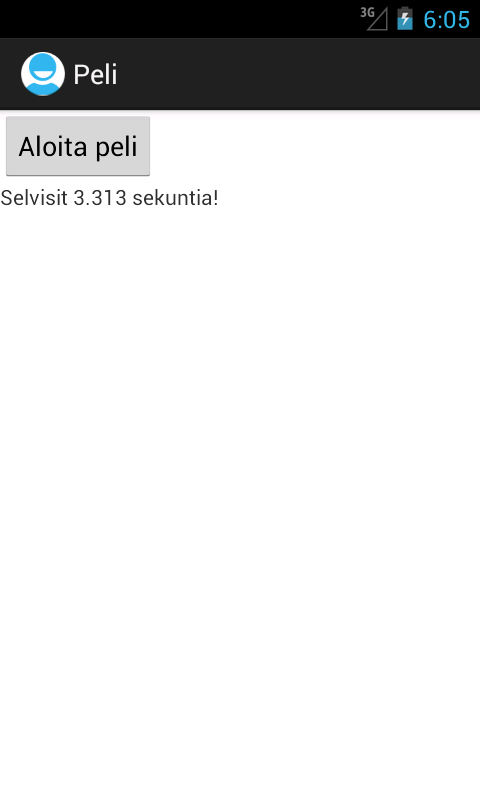
\includegraphics[width=60mm]{peli_mainactivity.png}}
\caption{Testiohjelman päänäkymä} \label{mainactivity}
\end{figure}

Peli koostuu kahdesta aktiviteetista, yksinkertaisemmasta MainActivitysta sekä hieman monimutkaisemmasta GameActivitysta, jonka yksikkötestaukseen keskityn. Itse peliä ohjaa GameView-luokka, joka on yhtä aikaa näkymä ja kontrolleri MVC-suunnittelumallin mukaisesti. Malleja ovat GameClock, joka kuvaa pelikelloa, sekä Circle, joka kuvaa yhtä ruudulla näkyvää ympyrää. GameActivity toteuttaa lisäksi OnGameEndListener-rajapinnan, jonka avulla GameView ilmoittaa pelin päättymisestä ja pistemäärästä. Pelin luokkakaavio on esitetty kuvassa \ref{game_classdiagram}.

\begin{figure}[h]
\centering
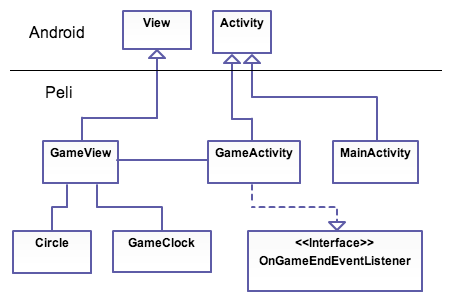
\includegraphics[width=105mm]{peli_luokkakaavio.png}
\caption{Testiohjelman luokkakaavio} \label{game_classdiagram}
\end{figure}

\subsection{Robolectricin asentaminen}
\label{robolectric_install}

Robolectricin suositeltu asennustapa on Maven, joka on yleisesti käytössä oleva kääntämis- ja riippuvuuksienhallintatyökalu \cite{maven}. Koska testattava projekti ei ollut Maven-projekti, jouduin tekemään Robolectric-testitkin ilman Mavenia. Ilman Mavenia asennus osoittautui haastavaksi: eri kirjastopakettien riippuvuudet eivät tahtoneet mitenkään toimia yhteen. Lopulta asennus kuitenkin onnistui tekemällä Robolectricin TestRunnerista oma aliluokka. Listauksessa \ref{robolectric_runner} on muokattu Robolectricin aliluokka testejä varten lähteenä olleesta esimerkistä \cite{sample_runner}. Olennaista on, että yliluokalle syötetään konstruktoriparametrina RobolectricConfig-olio, jolle annetaan parametrina testattavan Android-sovelluksen AndroidManifest.xml sekä resurssi-hakemiston osoite.

\begin{lstlisting}[float,label=robolectric_runner,caption=CustomRobolectricTestRunner]
public class CustomRobolectricTestRunner extends RobolectricTestRunner {
  public CustomRobolectricTestRunner(@SuppressWarnings("rawtypes") Class testClass) throws InitializationError {
  	super(testClass, new RobolectricConfig(new File("../Demo/AndroidManifest.xml"), new File("../Demo/res")));
  }
}
\end{lstlisting}

Robolectric-testejä varten luodaan oma tavallinen Java-projekti Eclipsessä, joka laitetaan viittaamaan Android-projektin koodiin. Testiprojektin käännöspolkuun tarvitaan Robolectricin jar-paketti, sekä Androidin android.jar sekä maps.jar -paketit. Robolectricin paketin pitää olla riippuvuuslistassa ennen Android-paketteja, jotta se toimii. Tämän jälkeen testejä voi ohjelmoida kuten tavallisia JUnit-testejä.

\subsection{Aktiviteetin elinkaarimetodien yksikkötestaus}
\label{basic_unittests} 

\begin{lstlisting}[float,label=robolectric_activitytest,caption=Yksinkertainen aktiviteettiyksikkötesti Robolectricilla]
@RunWith(CustomRobolectricTestRunner.class)
public class GameActivityTest {

  private GameActivity activity;

  @Before
  public void setUp() {
    activity = new GameActivity();
    activity.onCreate(null);
  }

  @Test
  public void testActivityInitializesViewWithRunningState() throws Exception {
    GameView gameView = (GameView) activity.findViewById(R.id.gameview);
    assertThat(gameView.getState(), equalTo(GameState.RUNNING));
  }
  
  @Test
  public void testOnPauseStopsTheGame() {
  	activity.onPause();
  	GameView gameView = (GameView) activity.findViewById(R.id.gameview);
  	assertThat(gameView.getState(), equalTo(GameState.PAUSED));
  }
  
}
\end{lstlisting}

Aktiviteetin elinkaarimetodien testaus on olennaisin osa Android-sovellusten yksikkötestauksesta. Listauksessa \ref{robolectric_activitytest} on yksinkertainen aktiviteettiyksikkötesti Robolectricillä toteutettuna. Robolectricin testit ovat yhteensopivia JUnitin 4. version kanssa, mikä mahdollistaa annotaatioiden käytön testeissä. @RunWith-annotaatiolla määritellään testien ajossa käytettävä testiajuri (\emph{runner}). Testissä käytetään luvussa \ref{robolectric_install} esiteltyä ajuria. @Before-annotaatiolla ilmaistaan metodit, jotka on ajettava ennen testejä ja @Test-annotaatiolla ajettavat testit.

setUp()-metodissa alustetaan testattava aktiviteetti ja kutsutaan sen onCreate()-metodia. Robolectric havaitsee automaattisesti Androidin kirjastometodien kutsun ja korvaa ne Robolectricin toteutuksella, jotta ne toimivat testissä. Siksi aktiviteetti voidaan alustaa suoraan konstruktorilla ja kutsua sen onCreate()-metodia toisin kuin AndroidUnitTestissä, jossa aktiviteetti käynnistetään AndroidUnitTestCase-luokan tarjoamien apumetodien avulla.

Ensimmäisessä testissä testataan, että aktiviteetin onCreate()-metodista alustetaan GameView-olio Running-tilaan. Robolectricin toteutus findViewById()-metodista mahdollistaa View-olion löytämisen Android-sovelluksen resursseissa määritellyn tunnisteen perusteella. Tämän jälkeen varmistetaan, että GameViewin tila on todella vaihtunut Running-tilaan. 

Toinen testi on rakenteeltaan hyvin samanlainen: siinä testataan, että onPause()-elinkaarimetodin kutsuminen siirtää GameViewin pause-tilaan. Testimekaniikka on sinänsä täsmälleen samanlainen kuin ensimmäisessä testissä.

Nämä testit eivät vaadi mitenkään ottamaan huomioon, että testejä tehdään Robolectriciä, eikä oikeaa Androidia vastaan. Robolectric toimii taustalla automaattisesti ja mahdollistaa testien vaatimat Androidin kirjastokutsut.

\begin{lstlisting}[float,label=androidunit_activitytest,caption=Yksinkertainen aktiviteettiyksikkötesti ActivityUnitTestCasen avulla]
public class GameActivityTest extends ActivityUnitTestCase<GameActivity> {

  private GameActivity activity;

  public GameActivityTest() {
  	super(GameActivity.class);
  }

  public void setUp() throws Exception {
  	super.setUp();
  	startActivity(new Intent(getInstrumentation().getTargetContext(), GameActivity.class), null, null);
    activity = (GameActivity)getActivity();
  }

  public void testActivityInitializesViewWithRunningState() {
    GameView gameView = (GameView) activity.findViewById(R.id.gameview);
    assertThat(gameView.getState(), equalTo(GameState.RUNNING));
  }
  
  public void testOnPauseStopsTheGame() {
  	activity.onPause();
  	GameView gameView = (GameView) activity.findViewById(R.id.gameview);
  	assertThat(gameView.getState(), equalTo(GameState.PAUSED));
  }
  
}
\end{lstlisting}

Listauksessa \ref{androidunit_activitytest} on toteutettu Androidin omalla yksikkötestikirjastolla vastaavat testit kuin listauksessa \ref{robolectric_activitytest}. Itse testit ovat täysin identtisiä Robolectric-testien välillä, erot ovat alustuksessa. Androidin aktiviteettiyksikkötestit perivät yliluokan ActivityUnitTestCase, jolle annetaan konstruktoriparametrina testattavan aktiviteetin luokka. Tämän jälkeen yliluokka instrumentoi luokan testausta varten.

setUp()-metodissa kutsutaan yliluokan setUp()-metodia ja käynnistetään testattava aktiviteetti yliluokan tarjoamalla startActivity()-metodilla. Tämän jälkeen viite testattavaan aktiviteettiin saadaan yliluokan getActivity()-metodilla.

Robolectricistä poiketen Androidin yksikkötestit ovat JUnit3-pohjaisia, joten annotaatioita ei käytetä, vaan metodien nimien perusteella päätellään setUp()-metodi sekä testimetodit siitä, että niiden nimi alkaa sanalla test. Koska JUnit3-testit kutsuvat testien alustamiseksi nimenomaan setUp()-nimistä metodia, on metodin alussa muistettava kutsua yliluokan setUp()-metodia, tai yliluokan suorittamat alustukset jäävät tekemättä.

\begin{lstlisting}[float,label=robolectric_shadow,caption=Aikeen tilatietojen tarkastelu Robolectricin varjo-olioilla]
@Test
public void testMainActivityIsCalledAfterLostGame() {
  GameView gameView = (GameView) activity.findViewById(R.id.gameview);
  gameView.setState(GameState.LOST);
  	
  ShadowActivity shadowActivity = shadowOf(activity);
  Intent startedIntent = shadowActivity.getNextStartedActivity();
  assertThat(startedIntent.getComponent().getClassName(), equalTo(MainActivity.class.getName()));
  assertThat(startedIntent.getStringExtra(GameActivity.SCORE), equalTo("0.0"));
}
\end{lstlisting}

Listauksessa \ref{robolectric_shadow} on hieman monimutkaisempi testitapaus Robolectricilla samasta testiluokasta kuin listaus \ref{robolectric_activitytest}. Tässä testissä testataan tapahtumia pelin loppuessa. Jos aktiviteetti toimii oikein, se rekisteröi GameView-oliolle havainnoija-suunnittelumallin (\emph{observer}) mukaisen havainnoijan, jota kutsutaan, kun peli päättyy. Aktiviteetin pitäisi tämän jälkeen pyytää GameView-oliolta pistemäärä ja lähettää uusi aie, jolla käynnistetään MainActivity-aktiviteetti ja annetaan aikeelle ylimääräisenä tietona saatu pistemäärä.

Androidin Activity-luokka ei tarjoa suoraa julkista metodia, jolla voitaisiin kysyä, minkä aikeen aktiviteetti on lähettänyt. Tällaisia tapauksia varten Robolectricilla on valmiina varjototeutus, joka kopioi oikean Android-luokan tilan ja tarjoaa laajemman mahdollisuuden aktiviteetin tilan kyselyyn. Tätä varten testissä tehdään varjo-olio testattavasta aktiviteetista, jolloin varjo-oliolta voidaan kysyä getNextStartedActivity()-metodilla, mikä on seuraava käynnistettävä aktiviteetti. Tältä aikeelta voidaan sitten tarkistaa, että aktiviteetti lähetti aikeen MainActivity-aktiviteetin käynnistämiseksi ja ylimääräisenä tietona on pistemäärä. Tässä tapauksessa pisteiden oletetaan olevan 0.0, koska pelikelloa ei missään testin vaiheessa käynnistetty.

\begin{lstlisting}[float,label=android_intent,caption=Aikeen tilatietojen tarkastelu ActivityUnitTestCasen avulla]
public void testMainActivityIsCalledAfterLostGame() {
  GameView gameView = (GameView) activity.findViewById(R.id.gameview);
  gameView.setState(GameState.LOST);
  	
  Intent startedIntent = getStartedActivityIntent();
  assertThat(startedIntent.getComponent().getClassName(), equalTo(MainActivity.class.getName()));
  assertThat(startedIntent.getStringExtra(GameActivity.SCORE), equalTo("0.0"));
}
\end{lstlisting}

Listauksessa \ref{android_intent} on toteutettu vastaava testi AndroidUnitTestCase:n avulla. Alustus tehdään testissä kuten Robolectric-testissäkin, mutta toiminnan varmistus on yksinkertaisempaa kuin Robolectricillä, koska AndroidUnitTestCase tarjoaa getStartedActivityIntent()-metodin, jolla saadaan aktiviteetin viimeisin lähettämä aie palautettua samalla tavalla kuin Robolectricin varjo-oliolta kysyttiin edellisessä listauksessa. Tämän jälkeen testin läpipääsyn varmistus tapahtuu täsmälleen samalla tavalla kuin Robolectric-testissä.

\subsection{Toiminta jäljittelijäkehysten kanssa}

Yksikkötestausta pyritään useimmiten tekemään niin, että testiluokka on eristetty riippuvuuksistaan. Apuvälineenä eristämisessä käytetään usein jäljittelijäkehyksiä. Näissä testeissä jäljittelijäkehyksenä käytetään Mockitoa, koska se toimii myös Androidissa sellaisenaan \cite{mockito}. Emulaattorissa ajamiseen tarvitsee vain Dalvik-käännöspaketin

Luvussa \ref{basic_unittests} esitetyt yksikkötestit ovat riippuvaisia GameView-luokan toteutuksesta. Testit voivat kuitenkin palauttaa virheellisen tuloksen, jos GameView-luokan setState()-metodi ei muutakaan onnistuneesti tilaa. Tällöin kyse on kuitenkin GameView-luokan, eikä GameActivity-luokan toiminnasta. GameActivityn osalta testissä ollaan oikeastaan vain kiinnostuneita siitä, että aktiviteetin käynnistyessä pelin tilaa yritetään muuttaa RUNNING-tilaan.

\begin{lstlisting}[float,label=mock_subclass, caption=Jäljittelijäaliluokka]
private class MockGameActivity extends GameActivity {
	
	private GameView gameView;

  public MockGameActivity(GameView gameView) {
	  setView(gameView);
  }

  @Override
  public View findViewById(int id) {
	  return gameView;
  }
  
  public void setView(GameView gameView) {
    this.gameView = gameView
  }
}
\end{lstlisting}

Aktiviteetti on testissä eristettävä GameView:stä niin, että oikean näkymän sijaan se saa käyttöönsä jäljitellyn version näkymästä. Aktiviteetti käyttää findViewById()-metodia näkymän lataamiseen, koska se on alustettu layout-tiedostossa. Jotta tähän metodikutsuun pääsee väliin, täytyi aktiviteetille tehdä testiä varten aliluokka MockGameActivity, joka on esitetty listauksessa \ref{mock_subclass}. Aliluokka toteuttaa findViewById()-metodista version, joka palauttaa aina sille parametrina annetun näkymän, joka voi olla esimerkiksi jäljitelty näkymä. Tämä on yleinen tapa käyttää jäljittelijäkehyksiä riippuvuuksien eristämiseksi.

Tämän voisi Robolectricillä tehdä vaihtoehtoisesti siten, että toteuttaa oman varjoluokan Activity-luokasta, joka on kaikkien aktiviteettien yliluokka. Toteutuksen voi tehdä siten, että käyttää Robolectricin oletustoteutusta kaikkeen muuhun paitsi findViewById()-metodin toteutukseen \cite{robolectric}. Jäljittelijänäkymän injektointia varten tälle voisi tehdä myös oman set-metodin, jolla jäljitelty näkymä sijoitettaisiin palautettavaksi. Yllä esitetty testattavan luokan aliluokka on kuitenkin helpompi tapa toteuttaa sama asia, koska Robolectriciä ei tarvitse erikseen käskeä käyttämään varjoluokkana itse tehtyä toteutusta. Lisäksi aliluokkatoteutuksella on helpompi vaihdella, käytetäänkö testeissä oman aliluokan ilmentymää, vai varsinaisen testattavan luokan ilmentymää.

\begin{lstlisting}[float,label=mock_test_robolectric, caption=Jäljittelyä käyttävä testi Robolectrcicillä]
@Test
public void testActivityInitializesGameWithRunningStateWithMock() throws Exception {
	GameView gameView = mock(GameView.class);
	activity = new MockGameActivity(gameView);
	activity.onCreate(null);
	verify(gameView).setState(GameState.RUNNING);
}
\end{lstlisting}

Listauksessa \ref{mock_test_robolectric} on esitetty edellisen listauksen aliluokkaa käyttävä Robolectric-testi. Ensimmäisellä rivillä luodaan Mockiton jäljittelijäolio GameView-luokasta. Toisella rivillä luodaan testattavan aktiviteetin aliluokka, jolle syötetään jäljitelty näkymä konstruktoriparametrina. Sitten kutsutaan onCreate-metodia, kuten listauksen \ref{robolectric_activitytest} vastaavassa testissä. Testin läpäisy testataan Mockiton verify-metodilla, joka varmistaa, että parametrina annettua jäljittelijäolion annettua metodia kutsuttiin annetulla parametrillä.

\begin{lstlisting}[float,label=mock_test_android, caption=Jäljittelyä käyttävä testi AndroidUnitTestillä]
public void testActivityInitializesGameWithRunningStateWithMock() throws Exception {
	GameView gameView = mock(GameView.class);
	MockGameActivity.setView(gameView);
	startActivity(new Intent(getInstrumentation().getTargetContext(), MockGameActivity.class), null, null);
	verify(gameView).setState(GameState.RUNNING);
}
\end{lstlisting}

AndroidUnitTestin avulla tehty vastaava testi listauksessa \ref{mock_test_android} on jäljittelijänäkymän luomisen ja testin läpäisyn varmistamisen kannalta täsmälleen samanlainen kuin Robolectric-testi. Testissä käytetään apuna vastaavaa aliluokkaa kuin Robolectric-testissäkin, mutta näkymä pitää syöttää aliluokalle setView()-metodissa, koska AndroidUnitTestille annetaan testattavan luokan nimi jo luokan määrittelyssä ja aktiviteetti käynnistetään yliluokan avulla jo ennen testeihin pääsyä.

\subsection{Testisyklin nopeus}

Robolectricin vahvuudeksi mainitaan toistuvasti sen testien ajonopeus. Testien ajonopeudella on merkitystä kahdesta syystä: ensinnäkin laajojen projektien tapauksessa testitapauksia voi olla hyvin paljon ja kaikkien testien ajo voi kestää hyvin pitkään, mikä hidastaa koodin jakamista tai ohjelmistotuotantoprosessia, kun muutosten regressiotestaus aiemmin tehtyjen yksikkötestien avulla kestää pitkään. Toiseksi kehitettäessä sovellusta esimerkiksi Mobile-D-prosessin mukaisesti testilähtöisesti osaa testejä ajetaan jatkuvasti. Prosessi pysähtyy aina testien ajoajaksi, joten jos yksittäisten testien ajaminen on kovin hidasta, ei testilähtöinen kehittäminen ole järkevää.

\begin{table}[h]
\centering
\begin{tabular}{ l l l l }
   & Keskiarvo (s) & Max (s) & Min (s) \\
  Robolectric & 1,59 & 1,61 & 1,577 \\
  AndroidUnitTest & 44,10 & 44,271 & 43,868 \\
\end{tabular}
\caption{Testisarjan kestot Robolectricilla ja AndroidUnitTestillä}
\label{unittest_timing}
\end{table}

Testasin ensin isomman testisetin ajonopeutta. Kopioin aiemmin luvussa esitellyn testiluokan jäljittelijätestin kanssa 32 erilliseksi testiluokaksi niin, että testimetodeita kertyi yhteensä 128. Ajoin kaikki testit yhtenä sarjana ja annoin Eclipsen ottaa aikaa testien suorituksesta. Tähän aikaan ei sisälly sitä aikaa, joka kuluu JUnitin käynnistymiseen, vain itse testien suoritusaika. Toistin testit viisi kertaa ja testikestojen keskiarvo, maksimi ja minimi on esitetty taulukossa \ref{unittest_timing}. Testit ajoin Macbook Pro:lla OS X versiolla 10.7.5, joka oli varustettu 2,7Ghz Intel core i7 -tuplaydinprosessorilla ja 8 gigatavun muistilla.

Robolectricin testisarja kesti keskimäärin 1,59 sekuntia, AndroidUnitTestilla 44,10 sekuntia. Testisarjan ajaminen emulaattorissa oli siis noin 27 kertaa hitaampaa kuin Robolectricilla JVM:llä. Koska testattava sovellus ja itse testit ovat hyvin yksinkertaisia, on aikaero todennäköisesti vielä suurempi laajempaa sovellusta testattaessa. Robolectricin lupaus nopeammista yksikkötesteistä vaikuttaa siis toteutuvan.

Testisarjan keston lisäksi tutkin yksittäisten testien kestoja. Erityisen kauan emulaattorissa ajetuista testeistä kesti ensimmäisen testiluokan jäljittelijätesti. Sen ajo kesti jokaisella ajokerralla yli 12 sekuntia, eli yli 25\% koko testisarjan kestosta. Tämä johtuu siitä, että Mockito muokkaa ohjelman tavukoodia toimintaansa varten ja sen ensimmäinen alustus on hyvin hidas. Sama hitaus oli havaittavissa myös Robolectric-testeissä: ensimmäinen mock-testi kesti noin 0,3 sekuntia, mikä on noin 19\% koko Robolectric-testisarjasta. Suhteellinen hidastuminen on siis verrattavissa AndroidUnitTestillä ajettuihin testeihin.

Robolectricillä myös kaikkein ensimmäinen testi on suhteessa hyvin hidas, noin 0,5 sekuntia. Robolectric toimii tavukooditason muokkauksessa Mockiton tavoin instrumentoidessaan testattavaa sovellusta toimimaan Robolectricin varjototeutusten kanssa, joten ensimmäisen testin suhteellinen hitaus johtunee samasta syystä kuin Mockitolla.
Nämä seikat eivät kuitenkaan muuta kokonaiskuvaa siitä, että testien ajaminen on todella paljon nopeampaa Robolectricillä kuin AndroidUnitTestillä.

\begin{table}[h]
\centering
\begin{tabular}{ l l l }
   & Ensimmäisen testin alkuun (s) & Koko testisarjan loppuun \\
  Robolectric & 2,7 & 4,3 \\
  AndroidUnitTest & 36 & 80 \\
\end{tabular}
\caption{Testisarjan kesto alustus mukaanlukien}
\label{unittest_startup}
\end{table}

Toiseksi testasin, kuinka kauan kestää testikehyksen alustus siihen pisteeseen, että ensimmäinen testi lähtee ajautumaan koodimuutoksen jälkeen. Tämä tarkoittaa Android-tapauksessa sovelluksen asentamista emulaattoriin ja testikehyksen alustusta. Tulokset on esitetty taulukossa \ref{unittest_startup}. Alustusajat olivat merkittäviä. Robolectricillä testikehyksen alustus kestää jopa kauemmin kuin koko 128 testin sarjan ajo ja AndroidUnitTestilläkin lähes yhtä kauan. Yhdenkin testin ajaminen AndroidUnitTestillä kestää yli 30 sekuntia.

\subsection{Yksikkötestauksen haasteita}

\begin{lstlisting}[float, label=tomdroid_example,caption=Tomdroid-koodiesimerkki]
public class EditNote extends ActionBarActivity {
  ...
  protected void onCreate(Bundle savedInstanceState) {
    ...
    content = (EditText) findViewById(R.id.content);
    ...
    Intent intent = getIntent();
    uri = intent.getData();
  }  
  
  public void onResume(){
    ...
    if (uri == null) {
  	  ...
    } else handleNoteUri(uri);
  }

  private void handleNoteUri(final Uri uri) {
    ...
    note = NoteManager.getNote(this, uri);
    if(note != null) {
      noteContent = note.getNoteContent(noteContentHandler);
    }
  }
  
  private Handler noteContentHandler = new Handler() {
    ...
    public void handleMessage(Message msg) {
      ...
      if(msg.what == NoteContentBuilder.PARSE_OK) {
      	showNote(false);
      	...
      }
      ...
    }
  }
  
  private void showNote(boolean xml) {
    ...
    content.setText(noteContent, TextView.BufferType.SPANNABLE);
    ...
  }
}
\end{lstlisting}

Koodin laadun suhteen yksikkötestaus on herkkää: alunperin tarkoitukseni oli tehdä yksikkötestaus luvussa \ref{tomdroid} esiteltyä sovellusta vasten kuten toiminnallinen testauskin. Tämä ei kuitenkaan onnistunut, koska sovellusta ei ollut mitenkään tehty yksikkötestaus mielessä.

Aloitin yrittämällä testata muistikirjan muokkausnäkymässä, että aktiviteetin käynnistys lataa muistikirjan sisällön. Listauksessa \ref{tomdroid_example} näkyy EditNote-aktiviteetin koodi, joka liittyy muistikirjan sisällön asettamiseen. onCreate()-metodin sisältö on suoraviivainen: content-muuttuja alustetaan ja aikeelta pyydetään uri, joka on muistikirjan tunniste. onResume()-metodissa kutsutaan yksityistä handleNoteUri()-metodia. Tässä metodissa pyydetään muistikirja NoteManagerin staattisella getNote()-metodilla ja jos muistikirja löytyy, pyydetään muistikirjalta sen sisältö getNoteContent()-metodilla, joka ottaa parametrikseen käsittelijän, joka on EditNoten yksityinen sisäluokka. 

Tässä kohdassa aktiviteetti muuttuu mahdottomaksi testata eristettynä riippuvuuksistaan. Ensimmäinen ongelma on staattinen NoteManager, jota ei voi suoraan jäljitellä Androidissa toimivilla jäljittelijäkehyksillä. Tämä ongelma on kuitenkin kierrettävissä vähäisellä ohjelmakoodimuutoksella: kääritään staattinen kutsu EditNoteen tehtävään uuteen metodiin getNote(), joka voidaan sitten jäljitellä testissä jäljittelyaliluokassa kuten listauksessa \ref{mock_subclass} tehtiin.

Lopullinen este testaamiselle on kuitenkin kohta, jossa muistikirjalta pyydetään sen sisältö getNoteContent()-metodilla. Metodi toimii siten, että sille annetaan parametriksi käsittelijä, joka on EditNoten yksityinen sisäluokka. Tämän käsittelijän sisältä handleMessage()-metodista taas kutsutaan showNote()-metodia, joka asettaa tekstin käyttöliittymään. Onnistuin jäljittelemään tämänkin toiminnan siten, että Note-olio oli jäljitelty ja sen getNoteContent()-tyngästä kutsuttiin parametrina annetun käsittelijän handleMessage()-metodia. Tässä vaiheessa testi kaatui, koska oikeasti getNoteContent()-metodi on asynkroninen ja getNoteContent()-metodin palauttama noteContent ehditään asettaa ennen kuin käsittelijästä kutsutaan showNote()-metodia. Tässä vaiheessa yksinkertaista testiä varten oli kertynyt jäljittelijäkoodia useita kymmeniä rivejä ja totesin testaamisen epäkäytännölliseksi.

Tämä osoittaa, että ohjelmakoodin täytyy olla rakenteeltaan kelvollista ja luokkien ja metodien noudattaa mahdollisimman pitkälti yhden vastuun periaatetta (\emph{single responsibility principle}, ks. \cite[95-98]{agile_development}), jotta niiden yksikkötestaus on mahdollista. Lisäksi suurin hyöty yksikkötesteistä on ennen ohjelmakoodia kirjoitettuna, jolloin myös koodin rakenne pysyy helpommin testattavana.

\subsection{Analyysi}

\begin{table}[h]
\centering
\begin{tabular}{ l l l }
  Arvioitu osa-alue & AndroidUnitTest & Robolectric \\
  Toiminnallisuus & Hyvä & Hyvä \\
  Testien ajonopeus & Hidas & Nopea \\
  Oppimisen helppous & Helpohko & Helpohko \\
  Testien kirjoitusnopeus & Nopeahko & Nopeahko \\
\end{tabular}
\caption{Testityökalujen osa-alueiden arviot}
\label{unittest_evaluation}
\end{table}

Ohjelmakoodin yksikkötestaus onnistui hyvin sekä Androidin mukana tulevalla yksikkötestikehyksellä, että Robolectricillä. Eri testattujen osa-alueiden yhteenveto on koottu taulukkoon \ref{unittest_evaluation}. Itse testikoodi ei poikennut kovin merkittävästi toisistaan eri kehyksille kirjoitetulla koodilla ja testien kirjoitukseen ei tarvinnut kovin paljoa Android-spesifiä osaamista. Robolectric-koodi oli jopa yksinkertaisempaa testattavien komponenttien alustuksen ostalta, koska konstruktoreja saattoi käyttää suoraan yliluokan tarjoamien alustusmetodien sijaan. Toisaalta joskus oli vaikea tietää, mitä metodeita eri luokkien valmiit varjototeutukset tarjoavat. Näissä tapauksissa AndroidUnitTestCasen yliluokkametodit olivat käytössä selkeämpiä. Toisaalta Robolectric tarjoaa mahdollisuuden kirjoittaa itse omia varjoluokkia, joissa voi toteuttaa tynkiä Androidin kirjastoluokkien toiminnalle.

Jäljittelijäkehyksen käyttö onnistui ongelmitta sekä Robolectricillä että AndroidUnitTestCasella. Mockito toimi suoraan yhdessä Robolectricin kanssa ja Android-emulaattorissa ajaminenkin onnistui helposti.

Suurin ero testityökalujen välillä oli testien suoritusnopeudessa. Robolectric lupaa nopeita testejä ja toteuttaa lupauksensa; Robolectric-testit ajautuivat yli 25 kertaa nopeammin kuin emulaattorissa ajetut AndroidUnitTestit. Lisäksi AndroidUnitTestillä aika ensimmäiseen testitulokseen pienelläkin testiohjelmalla oli yli puoli minuuttia, joten testilähtöinen ohjelmointi AndroidUnitTestCasea käyttäen on käytännössä toivottoman hidasta.

Tässä luvussa testattu sovellus oli hyvin yksinkertainen, joten jotkin tulokset eivät välttämättä skaalaudu suoraan suurempien sovellusten testaamiseen. Toisaalta yksikkötestauksessa pyritään yleensä riippuvuuksien rajaamiseen ja mahdollisimman pienten osien testaamista erikseen, joten periaatteessa suurempien sovellusten yksikkötestaaminen ei ole juuri vaikeampaa kuin yksinkertaisten. 

Toinen kysymys on ylipäänsä aktiviteettien yksikkötestauksen mielekkyys. Hyvin rakennetussa sovelluksessa sovelluslogiikka on eriytetty käyttöliittymälogiikasta omiin luokkiinsa, joten sovelluslogiikan yksikkötestaus onnistuu myös tavallisella JUnitilla. Sovelluslogiikassa useimmiten on myös testauksen kannalta tärkeimmät osat. Käyttöliittymälogiikan yksikkötestausta tehokkaampaa voisi sen sijaan olla suora toiminnallinen testaus käyttöliittymän kautta.